\ylDisplay{Kodarad} % Ülesande nimi
{Tundmatu autor} % Autor
{lahtine} % Voor
{2011} % Aasta
{G 10} % Ülesande nr.
{9} % Raskustase
{
% Teema: Kinemaatika
\ifStatement
\begin{wrapfigure}[8]{r}{40mm}
	\vspace{-10pt}
	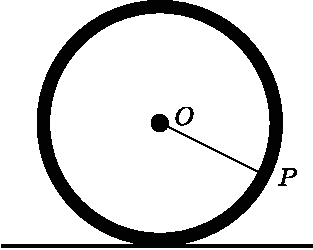
\includegraphics[width=40mm]{2011-lahg-10-kodar.pdf}
\end{wrapfigure}
Radiaalsete kodaratega rattast, mis veereb horisontaalsel pinnal, tehakse pilt.
Fotokaamera säriaeg on mõõduka pikkusega: paigalseisvad objektid on pildil teravad, 
liikuvad esemed aga hägused. Muuhulgas on ratta kodarad valdavalt hägusad, 
kuid osa kodarate teatud punktid on ometigi teravad. Võite eeldada, et kogu pilt on 
salvestatud samaaegselt. 
\\
\osa Kopeerige juuresolev skeem lahenduslehele ning näidake konstruktsiooni teel, 
milline kodara $OP$ punkt (või punktid) kujutub fotol teravalt; põhjendage vastust.\\
\osa Konstrueerige kõver, millel asuvad ülejäänud kodarate teravalt kujutuvad punktid.
\fi


\ifHint
Pildistamise hetkel pöörleb kogu ratas ümber hetkelise pöörlemistelje, mis läbib
ratta ja maa puutepunkti. See tähendab, et iga ratta osake liigub mööda ringjoone kaart, mille keskpunktiks on ratta ja maa puutepunkt.
\fi


\ifSolution
Kodara antud punkt näib kujutisel terav, kui selle kiirusvektor on suunatud pikki kodarat, st antud punktis kodar ei liigu enese ristsihis.

\begin{wrapfigure}{r}{0.3\textwidth}
	\vspace*{-15pt}
	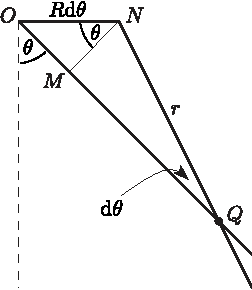
\includegraphics[width=0.3\textwidth]{2011-lahg-10-kodar_a}
	\vspace*{-25pt}
\end{wrapfigure}

Olukorda võib selgitada juuresoleva joonise abil.
Olgu $R$ ratta raadius ja olgu selle keskpunt $O$. Kui kodara pöördenurk on $\theta$ ning see nurk muutub pildistamise jooksul nurga $\D\theta$ võrra,
siis $O$ on läbinud teatud vahemaa ($R \, \D\theta$), aga kodar on samuti pöördunud sama nurga ($\D \theta$) võrra.
Jooniselt on näha, et uuel ja vanal kodara asendil on üks ühine punkt, olgu see punkt $Q$. Nii pildistamise alg- kui ka lõpphetkel asus selles punktis kodar, mistõttu kujutisel jääb see punkt selgelt näha (erinevalt teistest punktidest, kus kodar viibis vaid lühiajaliselt).

Kasutades eeltoodud joonist (kus tähistasime $OQ = r$) võime avaldada lõigu $MN$
pikkuse kahel viisil: $R \,\D \theta \cos \theta = r \,\D \theta$, kus
paremal pool kasutasime väikese nurga lähendust $\sin \D\theta\approx \D\theta$. Seega $R \cos \theta = r$, mis tähendab, et
(a) punkt $Q$ on leitav kodara lõikepunktina ratta ja maa kontaktpunktist $S$ kodarale tõmmatud ristsirgega (vt järgnev joonis);
(b) vaadeldes seda võrdust kui raadiuse $r$ sõltuvust polaarnurgast $\theta$ näeme, et ülejäänud kodarate teravalt kujutuvad punktid asuvad ringjoonel,
mille diameetriks on ratta raadius $OS$.

\vspace{0.5\baselineskip}

\textit{Alternatiivne lahendus}

Pildistamise hetkel pöörleb kogu ratas ümber hetkelise pöörlemistelje, mis läbib
ratta ja maa puutepunkti $S$ (vt. joonist). Sellel hetkel liigub iga ratta osake
mööda ringjoone kaart, mille keskpuntiks on $S$. Kui ühe sellisel moel liikuva
punkti kiirus on mööda kodarat ($OP$), siis see punkt kujutub fotol selgena.
Seega me otsime selliseid punkte $Q$, mille juures $\angle OQS$ on täisnurk.
Piirdenurga omaduse põhjal peab selline punkt $Q$ lebama ringjoonel, mille
diameetriks on $OS$ --- sõltumata kodara kaldenurgast $\theta$.
\begin{center}
	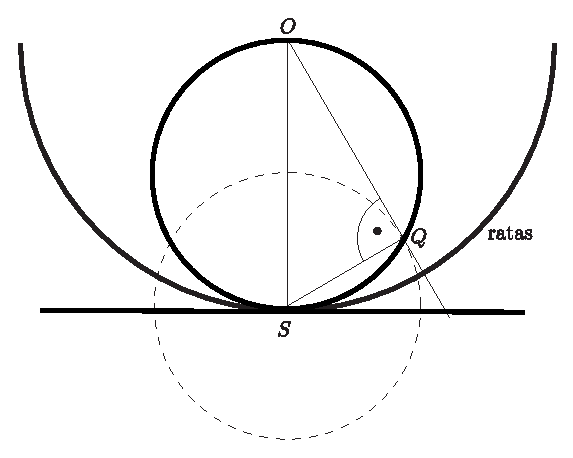
\includegraphics[width=0.65\textwidth]{2011-lahg-10-kodar_b}
\end{center}
\fi
}